%%%%%%%%%%%%%%%%%%%%%%%%%%%%%%%%%%%%%%%%%%%%%%%%%%%%%%%%
%%
\clearpage
\newpage
\section{The cal\_extract recipes}
\label{ch:the_recipes:cal_extract_RAW_spirou}
%%
%%%%%%%%%%%%%%%%%%%%%%%%%%%%%%%%%%%%%%%%%%%%%%%%%%%%%%%%

Extracts orders for specific fibers and files. There are currently three extraction recipes. There is the main extraction recipe (\calextractRAW) and two wrapper recipes (\calextractRAWAB and \calextractRAWC, which push certain options into \calextractRAW).

% -------------------------------------------------------
\subsection{The inputs}
% -------------------------------------------------------
The input of \calextractRAW is as follows:
\begin{cmdbox}
cal_extract_RAW_spirou.py night_repository filenames
\end{cmdbox}
\noindent for example
\begin{cmdbox}[title={example}]
cal_extract_RAW_spirou.py 20170710 fp_fp02a203.fits
\end{cmdbox}
\noindent or
\begin{pythonbox}
import cal_extract_RAW_spirou
night_repository = '20170710'
filenames = ['fp_fp02a203.fits']
cal_extract_RAW_spirou.main(night_repository, files=filenames)
\end{pythonbox}

\noindent where `night\_repository' defines \argnightname and `filenames' define the list of files in \argfilenames. In addition to this one can add optional arguments (and this is the case for the wrapper recipes of \calextractRAWAB and \calextractRAWC). \\

\noindent All files in filenames must be valid python strings separated by a space (command line) or in a line (python) and should have the following prefixes:
\begin{itemize}
	\item fp\_fp
	\item hcone\_dark
	\item dark\_hcone
	\item hcone\_hcone
	\item dark\_dark\_AHC1
	\item dark\_hctwo
	\item hctwo\_hctwo
	\item dark\_dark\_AHC2
\end{itemize}

\subsubsection{Optional arguments}

By default \calextractRAW will extract all fibers defined in \definevariable{text:fiber_types}{fiber\_types} (i.e. `AB', `A', `B' and `C'). It may be the case that one wishes to extract only one fiber, this can be done by setting the `fiber\_type' option (when run from python). For example:
\begin{pythonbox}
import cal_extract_RAW_spirou
night_repository = '20170710'
filenames = ['fp_fp02a203.fits']
cal_DARK_spirou.main(night_repository, filenames, fiber_type='A')
\end{pythonbox}
\noindent where `fiber\_type' must be a valid python string and defined in \definevariable{text:fiber_types}{fiber\_types}. On can also overwrite any other variable that is (or even is not) defined in any of the constant files (or run time) by simply adding it as an optional argument in the python function call:
\begin{pythonbox}
import cal_extract_RAW_spirou
night_repository = '20170710'
filenames = ['fp_fp02a203.fits', 'fp_fp03a203.fits', 'fp_fp04a203.fits']
kwargs = dict(parameter1='This', parameter2='That')
cal_DARK_spirou.main(night_repository, filenames, fiber_type='A', **kwargs)
\end{pythonbox}
\begin{note}
This will extract fiber `A' and also set the values \lstinline[style=pythoninline]|parameter1='This'| and \lstinline[style=pythoninline]|parameter2='That'| in the main constant parameter dictionary.
\end{note}
\noindent This is the case for the two wrapper recipes (\calextractRAWAB and \calextractRAWC) which add some specific keywords that are used to individually extract fibers `AB' and `C' respectively. The two calls to the main extraction code are shown below but can be called from the console or python as with all other recipes.
\begin{cmdbox}
cal_extract_RAW_spirouAB.py night_repository filenames
cal_extract_RAW_spirouC.py night_repository filenames
\end{cmdbox}
\noindent for example
\begin{cmdbox}[title={example}]
cal_extract_RAW_spirouAB.py 20170710 fp_fp02a203.fits fp_fp03a203.fits fp_fp04a203.fits
cal_extract_RAW_spirouC.py 20170710 fp_fp02a203.fits fp_fp03a203.fits fp_fp04a203.fits
\end{cmdbox}
\noindent or
\begin{pythonbox}
import cal_extract_RAW_spirouAB
import cal_extract_RAW_spirouC
night_repository = '20170710'
filenames = ['fp_fp02a203.fits']
# extract fiber AB
cal_extract_RAW_spirouAB.main(night_repository, files=filenames)
# extract fiber C
cal_extract_RAW_spirouC.main(night_repository, files=filenames)
\end{pythonbox}
\noindent as mentioned above this can also be done in python just by adding additional arguments to \calextractRAW:
\begin{pythonbox}
import cal_extract_RAW_spirou
night_repository = '20170710'
filenames = ['fp_fp02a203.fits', 'fp_fp03a203.fits', 'fp_fp04a203.fits']
# extract fiber AB (for all extraction types)
cal_extract_RAW_spirou.main(night_repository, files=filenames,fiber_type='AB',
                            ic_extract_type='all', ic_ext_sigdet=-1)
# extract fiber C (for all extraction types)
cal_extract_RAW_spirou.main(night_repository, files=filenames,fiber_type='C',
                            ic_extract_type='all', ic_ext_sigdet=-1)
\end{pythonbox}
\begin{note}
Here we set the optional arguments \lstinline[style=pythoninline]|ic_extract_type='all', ic_ext_sigdet=-1|. \definevariable{text:ic_extract_type}{ic\_extract\_type} defines which type of extraction should be used (simple, tilt, weigh, tiltweight, all) and \definevariable{text:ic_ext_sigdet}{ic\_ext\_sigdet} manually sets the extraction sigdet (-1 sets it to the value from the HEADER else it is defined in \constantsfile).
\end{note}
\noindent The above python code is exactly what \calextractRAWAB and \calextractRAWC do by default.


% -------------------------------------------------------
\subsection{The outputs}
% -------------------------------------------------------
The outputs of \calextractRAW depend on the extraction type (\definevariable{text:ic_extract_type}{ic\_extract\_type}). 

\begin{itemize}

\item \definevariable{text:e2ds_file}{e2ds} in form:
\begin{tcustomdir}
\{\reduceddir\}/\{date prefix\}\_\{file\}\_e2ds\_\{fiber\}.fits
\end{tcustomdir}

\item \definevariable{text:exfitslist}{simple} in form:
\begin{tcustomdir}
\{\reduceddir\}/\{date prefix\}\_\{file\}\_e2ds\_\{fiber\}\_simple.fits
\end{tcustomdir}
\begin{note}
Only if \definevariable{text:ic_extract_type}{ic\_extract\_type} is `all'
\end{note}

\item \definevariable{text:exfitslist}{tilt} in form:
\begin{tcustomdir}
\{\reduceddir\}/\{date prefix\}\_\{file\}\_e2ds\_\{fiber\}\_tilt.fits
\end{tcustomdir}
\begin{note}
Only if \definevariable{text:ic_extract_type}{ic\_extract\_type} is `all'
\end{note}

\item \definevariable{text:exfitslist}{tiltweight} in form:
\begin{tcustomdir}
\{\reduceddir\}/\{date prefix\}\_\{file\}\_e2ds\_\{fiber\}\_tiltweight.fits
\end{tcustomdir}
\begin{note}
Only if \definevariable{text:ic_extract_type}{ic\_extract\_type} is `all'
\end{note}

\item \definevariable{text:exfitslist}{tiltweight2} in form:
\begin{tcustomdir}
\{\reduceddir\}/\{date prefix\}\_\{file\}\_e2ds\_\{fiber\}\_tiltweight2.fits
\end{tcustomdir}
\begin{note}
Only if \definevariable{text:ic_extract_type}{ic\_extract\_type} is `all'
\end{note}

\item \definevariable{text:exfitslist}{weight} in form:
\begin{tcustomdir}
\{\reduceddir\}/\{date prefix\}\_\{file\}\_e2ds\_\{fiber\}\_weight.fits
\end{tcustomdir}
\begin{note}
Only if \definevariable{text:ic_extract_type}{ic\_extract\_type} is `all'
\end{note}

\end{itemize}


\noindent where `date prefix' is constructed from \argnightname and the file name is the first file in \argfilenames.


\noindent for example for \reduceddir\lstinline[style=pythoninline]|='/drs/data/reduced/20170710'| and \argfilenames\lstinline[style=pythoninline]|=['fp_fp02a203.fits']| and, \lstinline[style=pythoninline]|fiber_type='all'| the output files would be:
\begin{tcustomdir}
\begin{itemize}
\item \path{/drs/data/reduced/20170710/fp_fp02a203_e2ds_AB.fits}
\item \path{/drs/data/reduced/20170710/fp_fp02a203_e2ds_A.fits}
\item \path{/drs/data/reduced/20170710/fp_fp02a203_e2ds_B.fits}
\item \path{/drs/data/reduced/20170710/fp_fp02a203_e2ds_C.fits}
\end{itemize}
\end{tcustomdir}
\noindent or if \lstinline[style=pythoninline]|ic_extract_type='all'| and \lstinline[style=pythoninline]|fiber_type='AB'| the output files would be:
\begin{tcustomdir}
\begin{itemize}
\item \path{/drs/data/reduced/20170710/fp_fp02a203_e2ds_AB.fits}
\item \path{/drs/data/reduced/20170710/fp_fp02a203_e2ds_AB_simple.fits}
\item \path{/drs/data/reduced/20170710/fp_fp02a203_e2ds_AB_tilt.fits}
\item \path{/drs/data/reduced/20170710/fp_fp02a203_e2ds_AB_tiltweight.fits}
\item \path{/drs/data/reduced/20170710/fp_fp02a203_e2ds_AB_tiltweight2.fits}
\item \path{/drs/data/reduced/20170710/fp_fp02a203_e2ds_AB_weight.fits}
\end{itemize}
\end{tcustomdir}


% -------------------------------------------------------
\subsection{Summary of procedure}
% -------------------------------------------------------

\begin{enumerate}
\item adds all files together (if more than one)
\item corrects for darks
\item resizes the image
\item checks for saturation
\item possible background subtraction?
\item extracts orders (depending on \definevariable{text:ic_extract_type}{ic\_extract\_type})
	\begin{itemize}
		\item without tilt/weight Fortran
		\item without tilt/weight python
		\item with tilt (no weight)
		\item with tilt and weight
		\item with weight (no tilt)
	\end{itemize}
\item saves extraction to e2ds file(s)
\end{enumerate}


% -------------------------------------------------------
\subsection{Quality Control}
% -------------------------------------------------------

There is currently one quality control check for \calextractRAW
\begin{itemize}
\item Too much flux in the image: 
\begin{thighlight}
\begin{equation}
\text{maximum signal} > \text{\definevariable{text:qc_max_signal}{qc\_max\_signal}} * \text{\definevariable{text:nbframes}{nbframes}}
\end{equation}
\end{thighlight}
\end{itemize}
\begin{note}
This check does not currently lead to a failed run and all files are processed as passing quality checks
\end{note}

% -------------------------------------------------------
\subsection{Example working run}
% -------------------------------------------------------

An example run where everything worked is below:
\begin{cmdbox}[title={example}]
cal_extract_RAW_spirou.py 20170710 fp_fp02a203.fits
\end{cmdbox}
\begin{cmdboxprintspecial}[fontupper=\tiny, fontlower=\tiny]
@gHH:MM:SS.S -   || *****************************************@g
@gHH:MM:SS.S -   || * SPIROU \@(#) Geneva Observatory (VERSION)@g
@gHH:MM:SS.S -   || *****************************************@g
@gHH:MM:SS.S -   ||(dir_data_raw)      DRS_DATA_RAW=/drs/data/raw@g
@gHH:MM:SS.S -   ||(dir_data_reduc)    DRS_DATA_REDUC=/drs/data/reduced@g
@gHH:MM:SS.S -   ||(dir_calib_db)      DRS_CALIB_DB=/drs/data/calibDB@g
@gHH:MM:SS.S -   ||(dir_data_msg)      DRS_DATA_MSG=/drs/data/msg@g
@gHH:MM:SS.S -   ||(print_level)       PRINT_LEVEL=all         %(error/warning/info/all)@g
@gHH:MM:SS.S -   ||(log_level)         LOG_LEVEL=all         %(error/warning/info/all)@g
@gHH:MM:SS.S -   ||(plot_graph)        DRS_PLOT=1            %(def/undef/trigger)@g
@gHH:MM:SS.S -   ||(used_date)         DRS_USED_DATE=undefined@g
@gHH:MM:SS.S -   ||(working_dir)       DRS_DATA_WORKING=/drs/data/tmp@g
@gHH:MM:SS.S -   ||                    DRS_INTERACTIVE is not set, running on-line mode@g
@gHH:MM:SS.S -   ||                    DRS_DEBUG is set, debug mode level:1@g
@gHH:MM:SS.S -   |cal_extract_RAW_spirou:2a203|Now running : cal_extract_RAW_spirou on file(s): fp_fp02a203.fits@g
@gHH:MM:SS.S -   |cal_extract_RAW_spirou:2a203|On directory /drs/data/raw/20170710@g
@gHH:MM:SS.S -   |cal_extract_RAW_spirou:2a203|ICDP_NAME loaded from: /scratch/Projects/spirou_py3/spirou_py3/INTROOT/config/constants_SPIROU.py@g
@gHH:MM:SS.S -   |cal_extract_RAW_spirou:2a203|Calibration file: 20170710_flat_flat02f10_badpixel.fits already exists - not copied@g
...
@gHH:MM:SS.S -   |cal_extract_RAW_spirou:2a203|Calibration file: 2017-10-11_21-32-17_hcone_hcone02c406_wave_C.fits already exists - not copied@g
@gHH:MM:SS.S - * |cal_extract_RAW_spirou:2a203|Now processing Image TYPE UNKNOWN with cal_extract_RAW_spirou recipe@g
@gHH:MM:SS.S -   |cal_extract_RAW_spirou:2a203|Reading Image /drs/data/raw/20170710/fp_fp02a203.fits@g
@gHH:MM:SS.S -   |cal_extract_RAW_spirou:2a203|Image 2048 x 2048 loaded@g
@gHH:MM:SS.S -   |cal_extract_RAW_spirou:2a203|Doing Dark Correction using /drs/data/calibDB/20170710_dark_dark02d406.fits@g
@gHH:MM:SS.S -   |cal_extract_RAW_spirou:2a203|Image format changed to 2035x1930@g
@gHH:MM:SS.S - * |cal_extract_RAW_spirou:2a203|Nb dead pixels = 568485 / 14.47 %@g
@gHH:MM:SS.S - * |cal_extract_RAW_spirou:2a203|Maximum average flux/pixel in the spectrum: 109726.7 [ADU]@g
@gHH:MM:SS.S -   |cal_extract_RAW_spirou:2a203|Reading localization parameters of Fiber AB@g
@gHH:MM:SS.S -   |cal_extract_RAW_spirou:2a203AB|Reading order profile of Fiber AB@g
@gHH:MM:SS.S -   |cal_extract_RAW_spirou:2a203|On fiber AB order 0: S/N= 352.4@g
@gHH:MM:SS.S -   |cal_extract_RAW_spirou:2a203|On fiber AB order 1: S/N= 398.4@g
...
@gHH:MM:SS.S -   |cal_extract_RAW_spirou:2a203|On fiber AB order 34: S/N= 138.8@g
@gHH:MM:SS.S -   |cal_extract_RAW_spirou:2a203|On fiber AB order 35: S/N= 47.8@g
@gHH:MM:SS.S -   |cal_extract_RAW_spirou:2a203|Saving E2DS spectrum of Fiber AB in fp_fp02a203_e2ds_AB.fits@y
@yHH:MM:SS.S - \@ |python warning Line 980  warning reads: Card is too long, comment will be truncated.|@g
@gHH:MM:SS.S -   |cal_extract_RAW_spirou:2a203|Reading localization parameters of Fiber A@g
@gHH:MM:SS.S -   |cal_extract_RAW_spirou:2a203A|Reading order profile of Fiber A@g
@gHH:MM:SS.S -   |cal_extract_RAW_spirou:2a203|On fiber A order 0: S/N= 210.2@g
@gHH:MM:SS.S -   |cal_extract_RAW_spirou:2a203|On fiber A order 1: S/N= 237.4@g
...
@gHH:MM:SS.S -   |cal_extract_RAW_spirou:2a203|On fiber A order 34: S/N= 114.3@g
@gHH:MM:SS.S -   |cal_extract_RAW_spirou:2a203|On fiber A order 35: S/N= 33.8@g
@gHH:MM:SS.S -   |cal_extract_RAW_spirou:2a203|Saving E2DS spectrum of Fiber A in fp_fp02a203_e2ds_A.fits@g
@yHH:MM:SS.S - \@ |python warning Line 980  warning reads: Card is too long, comment will be truncated.|@y
@gHH:MM:SS.S -   |cal_extract_RAW_spirou:2a203|Reading localization parameters of Fiber B@g
@gHH:MM:SS.S -   |cal_extract_RAW_spirou:2a203B|Reading order profile of Fiber B@g
@gHH:MM:SS.S -   |cal_extract_RAW_spirou:2a203|On fiber B order 0: S/N= 286.8@g
@gHH:MM:SS.S -   |cal_extract_RAW_spirou:2a203|On fiber B order 1: S/N= 324.4@g
...
@gHH:MM:SS.S -   |cal_extract_RAW_spirou:2a203|On fiber B order 34: S/N= 87.2@g
@gHH:MM:SS.S -   |cal_extract_RAW_spirou:2a203|On fiber B order 35: S/N= 36.1@g
@gHH:MM:SS.S -   |cal_extract_RAW_spirou:2a203|Saving E2DS spectrum of Fiber B in fp_fp02a203_e2ds_B.fits@g
@yHH:MM:SS.S - \@ |python warning Line 980  warning reads: Card is too long, comment will be truncated.|@y
@gHH:MM:SS.S -   |cal_extract_RAW_spirou:2a203|Reading localization parameters of Fiber C@g
@gHH:MM:SS.S -   |cal_extract_RAW_spirou:2a203C|Reading order profile of Fiber C@g
@gHH:MM:SS.S -   |cal_extract_RAW_spirou:2a203|On fiber C order 0: S/N= 376.6@g
@gHH:MM:SS.S -   |cal_extract_RAW_spirou:2a203|On fiber C order 1: S/N= 424.3@g
...
@gHH:MM:SS.S -   |cal_extract_RAW_spirou:2a203|On fiber C order 34: S/N= 252.7@g
@gHH:MM:SS.S -   |cal_extract_RAW_spirou:2a203|On fiber C order 35: S/N= 130.0@g
@gHH:MM:SS.S -   |cal_extract_RAW_spirou:2a203|Saving E2DS spectrum of Fiber C in fp_fp02a203_e2ds_C.fits@g
@yHH:MM:SS.S - \@ |python warning Line 980  warning reads: Card is too long, comment will be truncated.|@y
@gHH:MM:SS.S - * |cal_extract_RAW_spirou:2a203|Too much flux in the image (max authorized=65500)@g
@gHH:MM:SS.S - * |cal_extract_RAW_spirou:2a203|QUALITY CONTROL SUCCESSFUL - Well Done -@g
@gHH:MM:SS.S - * |cal_extract_RAW_spirou:2a203|Recipe cal_extract_RAW_spirou has been successfully complted@g
\end{cmdboxprintspecial}


% % -------------------------------------------------------
% \newpage
% \subsection{Interactive mode}
% % -------------------------------------------------------

% \noindent In interactive mode three figures will also appear (see Figure \ref{figure:}).

% \begin{figure}

% \begin{center}
% \begin{minipage}{.495\textwidth}
% \begin{center}
% \includegraphics[width=\textwidth]{Figures/cal_DARK_spirou_1.pdf}
% a
% \end{center}
% \end{minipage}%
% \begin{minipage}{.495\textwidth}
% \begin{center}
% \includegraphics[width=\textwidth]{Figures/cal_DARK_spirou_2.pdf}
% b
% \end{center}
% \end{minipage}%
% \end{center}

% \begin{center}
% \begin{minipage}{.495\textwidth}
% \begin{center}
% \includegraphics[width=\textwidth]{Figures/cal_DARK_spirou_3.pdf}
% c
% \end{center}
% \end{minipage}%
% \end{center}

% \caption{\textbf{(a)} The image with overplot red and blue regions (red/blue rectangles). \textbf{(b)} The bad pixel mask, bad pixels have a value=1 (in black) and good pixels have a value=0 (in white). \textbf{(c)} Histograms of the image regions, the full image (in green), the blue section (in blue) and the red section (in red). \label{figure:cal_DARK_spirou}}
% \end{figure}